\def\eps{.05}
\newcommand\lufactornodes[2]{
        \node [name=la] at (0,0.9) {};
        \node [name=da] at (0.1,0.9) {};
        \node [name=dau] at (0.1+#1,0.9+#2) {};
        \node [name=ua] at (1+#1,0.9+#2) {};
        \node [name=lb] at (0,0.7) {};
        \node [name=db] at (0.3,0.7) {};
        \node [name=dbu] at (0.3+#1,0.7+#2) {};
        \node [name=ub] at (1+#1,0.7+#2) {};
        \node [name=lc] at (0,0.5) {};
        \node [name=dc] at (0.5,0.5) {};
        \node [name=dcu] at (0.5+#1,0.5+#2) {};
        \node [name=uc] at (1+#1,0.5+#2) {};
        \node [name=ld] at (0,0.3) {};
        \node [name=dd] at (0.7,0.3) {};
        \node [name=ddu] at (0.7+#1,0.3+#2) {};
        \node [name=ud] at (1+#1,0.3+#2) {};
        \node [name=le] at (0,0.1) {};
        \node [name=de] at (0.9,0.1) {};
        \node [name=deu] at (0.9+#1,0.1+#2) {};
        \node [name=ue] at (1+#1,0.1+#2) {};
}
\newcommand\lufactors{
        \begin{scope}[color=red!90, ->]
          \draw [memread] (la) -- (da);
          \draw [memskip forward] (la) to[->,in=180] (da) to[in=135] (lb);
          \draw [memread] (lb) -- (db);
          \draw [memskip forward] (db) to (lc);
          \draw [memread] (lc) -- (dc);
          \draw [memskip forward] (dc) to (ld);
          \draw [memread] (ld) -- (dd);
          \draw [memskip forward] (dd) to (le);
          \draw [memread] (le) -- (de);
        \end{scope}
        \begin{scope}[color=blue!90, ->]
          \draw [memread] (ue) to (deu);
          \draw [memskip back] (ue) to[in=0] (deu) to[in=-45] (ud);
          \draw [memread] (ud) to (ddu);
          \draw [memskip back] (ddu) to (uc);
          \draw [memread] (uc) to (dcu);
          \draw [memskip back] (dcu) to (ub);
          \draw [memread] (ub) to (dbu);
          \draw [memskip back] (dbu) to (ua);
          \draw [memread] (ua) to (dau);
        \end{scope}
}

\begin{frame}{Storing Factors}
  \begin{columns}
    \begin{column}{0.3\textwidth}
      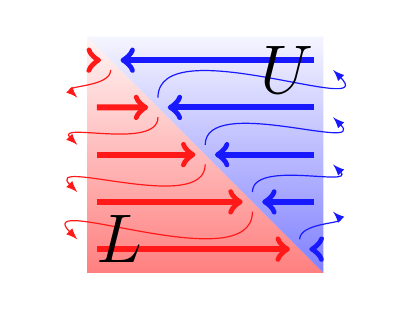
\begin{tikzpicture}[scale=3,
        memread/.style={line width=.5ex, >=to},
        memskip forward/.style={line width=.1ex, out=-90, in=135, >=latex},
        memskip back/.style={line width=.1ex, out=90, in=-45, >=latex}
        ]
        \shade [top color=red!4, bottom color=red!50] (0,1) -- (1,0) -- (0,0) -- cycle;
        \shade [top color=blue!4, bottom color=blue!50] (0,1) -- (1,0) -- (1,1) -- cycle;
        \lufactornodes{0}{0}
        \lufactors
        \node [anchor=south west, color=black] at (0,0) {\Huge $L$};
        \node [anchor=north east, color=black] at (1,1) {\Huge $U$};
      \end{tikzpicture}
    \end{column}
    \begin{column}{0.7\textwidth}
      \begin{itemize}
      \item Forward and back solves skip over unused part of each row
        \begin{itemize}
        \item Pollutes cache and bus with unused part, software prefetch helps some
        \end{itemize}
      \item Back solves move backward through memory and so does vector
        \begin{itemize}
        \item Core 2: hardware prefetch 16 forward-moving pointers and 4 backward-moving \\
          not across 4 KiB page boundaries
        \end{itemize}
      \end{itemize}
    \end{column}
  \end{columns}
  \begin{columns}
    \begin{column}{0.3\textwidth}
      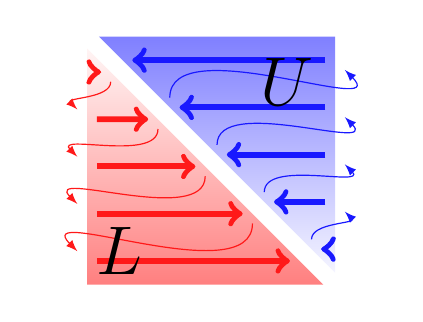
\begin{tikzpicture}[scale=3,
        memread/.style={line width=.5ex, >=to},
        memskip forward/.style={line width=.1ex, out=-90, in=135, >=latex},
        memskip back/.style={line width=.1ex, out=90, in=-45, >=latex}
        ]
        \shade [top color=red!4, bottom color=red!50] (0,1) -- (1,0) -- (0,0) -- cycle;
        \shade [top color=blue!50, bottom color=blue!4] (0.05,1.05) -- (1.05,0.05) -- (1.05,1.05) -- cycle;
        \lufactornodes{.05}{.05}
        \lufactors
        \node [anchor=south west, color=black] at (0,0) {\Huge $L$};
        \node [anchor=north east, color=black] at (1,1) {\Huge $U$};
      \end{tikzpicture}
    \end{column}
    \begin{column}{0.7\textwidth}
      \begin{itemize}
      \item Forward and back solves get contiguous memory
      \item Move forward through memory for matrix entries
        \begin{itemize}
        \item Good for vector prefetch which necessarily tracks backward through memory
        \end{itemize}
      \end{itemize}
    \end{column}
  \end{columns}
\end{frame}
